%==============================================================================
% Section 6: Three-Topology Comparison
%==============================================================================
\section{Three-Topology Comparison}
\label{sec:compare}

This section integrates the results of \S\S\ref{sec:s3}--\ref{sec:nil3} and
performs a systematic comparison across the three topologies
$\Sthree\times\Sone$, $\Tthree\times\Sone$, and $\Nilthree\times\Sone$.  The
main result is \textbf{Theorem~9 ($\varepsilon$-$s$ cross-term classification)};
the $\gamma=1/2$ scaling theorem and the conformal-flatness theorem complement it.

\subsection{Comparative Summary Table (Table~4)}
\label{sec:compare:table}

\begin{table}[H]
\centering
\resizebox{\linewidth}{!}{%
\begin{tabular}{lccc}
\toprule
Quantity & $\Tthree\times\Sone$ & $\Nilthree\times\Sone$ & $\Sthree\times\Sone$ \\
\midrule
EC slice min.\ on $\eta=V=0$ ($\alpha<0$) & absent & \textbf{present (new)} & absent \\
$C^2_\LC$ ($\eta=V=0$) & $0$ (flat) & $\mathbf{4/(3R^4)\neq 0}$ & $0$ (conf.\ flat) \\
Conformal flatness & \checkmark (flat) & $\times$ (\textbf{non-conf.\ flat}) & \checkmark (conf.\ flat) \\
Palatini protection & \checkmark & \checkmark & \checkmark \\
spin-2 (AX background) & $0$ (flatness) & non-zero mass & $128\pi^2 Lr/(3\kappa^2) - 16384\pi^2 L\alpha/(3r)$ \\
spin-1 structure & all zero & \textbf{uniaxial splitting} ($\omega_2$ only) & 3-fold degenerate \\
$\gamma_\EC$ & --- & $\mathbf{1/2}$ (exact) & --- \\
$\varepsilon$-$s$ cross-term & kinematic & curvature/Weyl & $0$ (vanishes) \\
\bottomrule
\end{tabular}%
}
\caption{Comparison of EC--Weyl effects across the three topologies.}
\label{tab:compare}
\end{table}

\subsection{Theorem~9: $\varepsilon$-$s$ Cross-term Classification}
\label{sec:compare:thm9}

\begin{theorem}[$\varepsilon$-$s$ cross-term classification]\label{thm:crossterm}
  The mixed second derivative of the squash parameter $\varepsilon$ and the
  shear parameter $s$, $\partial^2 V/\partial\varepsilon\partial s|_{\varepsilon=s=0}$,
  has an essentially different origin in the three topologies\textup{:}
  \begin{center}
  \resizebox{\linewidth}{!}{%
  \begin{tabular}{lccc}
  \toprule
  Topology & $\partial^2 V/\partial\varepsilon\partial s$ & Origin & Volume-preserving \\
  \midrule
  $\Tthree$ & $48\pi^4 L\eta^2 r/\kappa^2 \neq 0$ & \textbf{pure kinematic} (non-volume-pres.) & $\times$ \\
  $\Nilthree$ & $(384\pi^4 LR^2-8192\pi^4 L\alpha\kappa^2)/(9R\kappa^2)\neq 0$ & \textbf{pure curvature/Weyl} & \checkmark \\
  $\Sthree$ & $0$ (SymPy exact) & vanishes (volume-pres.\ + $s\to -s$ sym.) & \checkmark \\
  \bottomrule
  \end{tabular}%
  }
  \end{center}
\end{theorem}

\begin{proof}[Proof outline]
  The detailed derivation is given in Appendix~\ref{app:C}.  The three key
  points are as follows.
  \begin{itemize}
    \item $\Tthree$: The volume element $(1+\varepsilon)(1+s)$ is non-trivial,
          and despite $C^a_{bc}=0$ a purely kinematic cross-term arises
          (Theorem~\ref{thm:tvol}, Appendix~\ref{app:C:t3}).
    \item $\Nilthree$: Volume preservation holds, but the directional asymmetry
          of $C^2_{01}$ leaves an $\alpha$-dependent curvature/Weyl-origin
          cross-term (Appendix~\ref{app:C:nil3}).
    \item $\Sthree$: Volume preservation holds, and additionally the
          $s\to-s$ symmetry of the effective potential causes the cross-term to
          vanish (Appendix~\ref{app:C:s3}).
  \end{itemize}
  Script: \texttt{paper03ec/squash\_shear\_cross\_term.py}.
\end{proof}

\paragraph{Physical meaning.}
This classification maps the geometric properties of each topology (flatness,
conformal flatness, volume preservation, non-commutative structure) directly
onto the squash--shear cross-term as an observable.

\subsection{$\gamma = 1/2$ Scaling Theorem}
\label{sec:compare:gamma}

We establish the scaling exponent of the $\Nilthree\times\Sone$ EC slice minimum
analytically.

When the effective potential has the two-term structure
\begin{equation}
  \Veff = A\cdot r^n + \alpha\cdot B\cdot r^m,
\end{equation}
the general scaling relations are
\begin{equation}
  r_0 \propto |\alpha|^{1/(n-m)},
  \quad
  V^c \propto |\alpha|^{n/(n-m)},
  \quad
  \gamma = \frac{n}{n-m}.
\end{equation}
For $\Nilthree$, $n=1$ (power of the LC term) and $m=-1$ (power of the EC term),
so
\begin{equation}
  n - m = 2,
  \qquad
  \gamma = \delta = \frac{1}{2} \quad (\text{algebraically determined}).
\end{equation}

\begin{figure}[H]
  \centering
  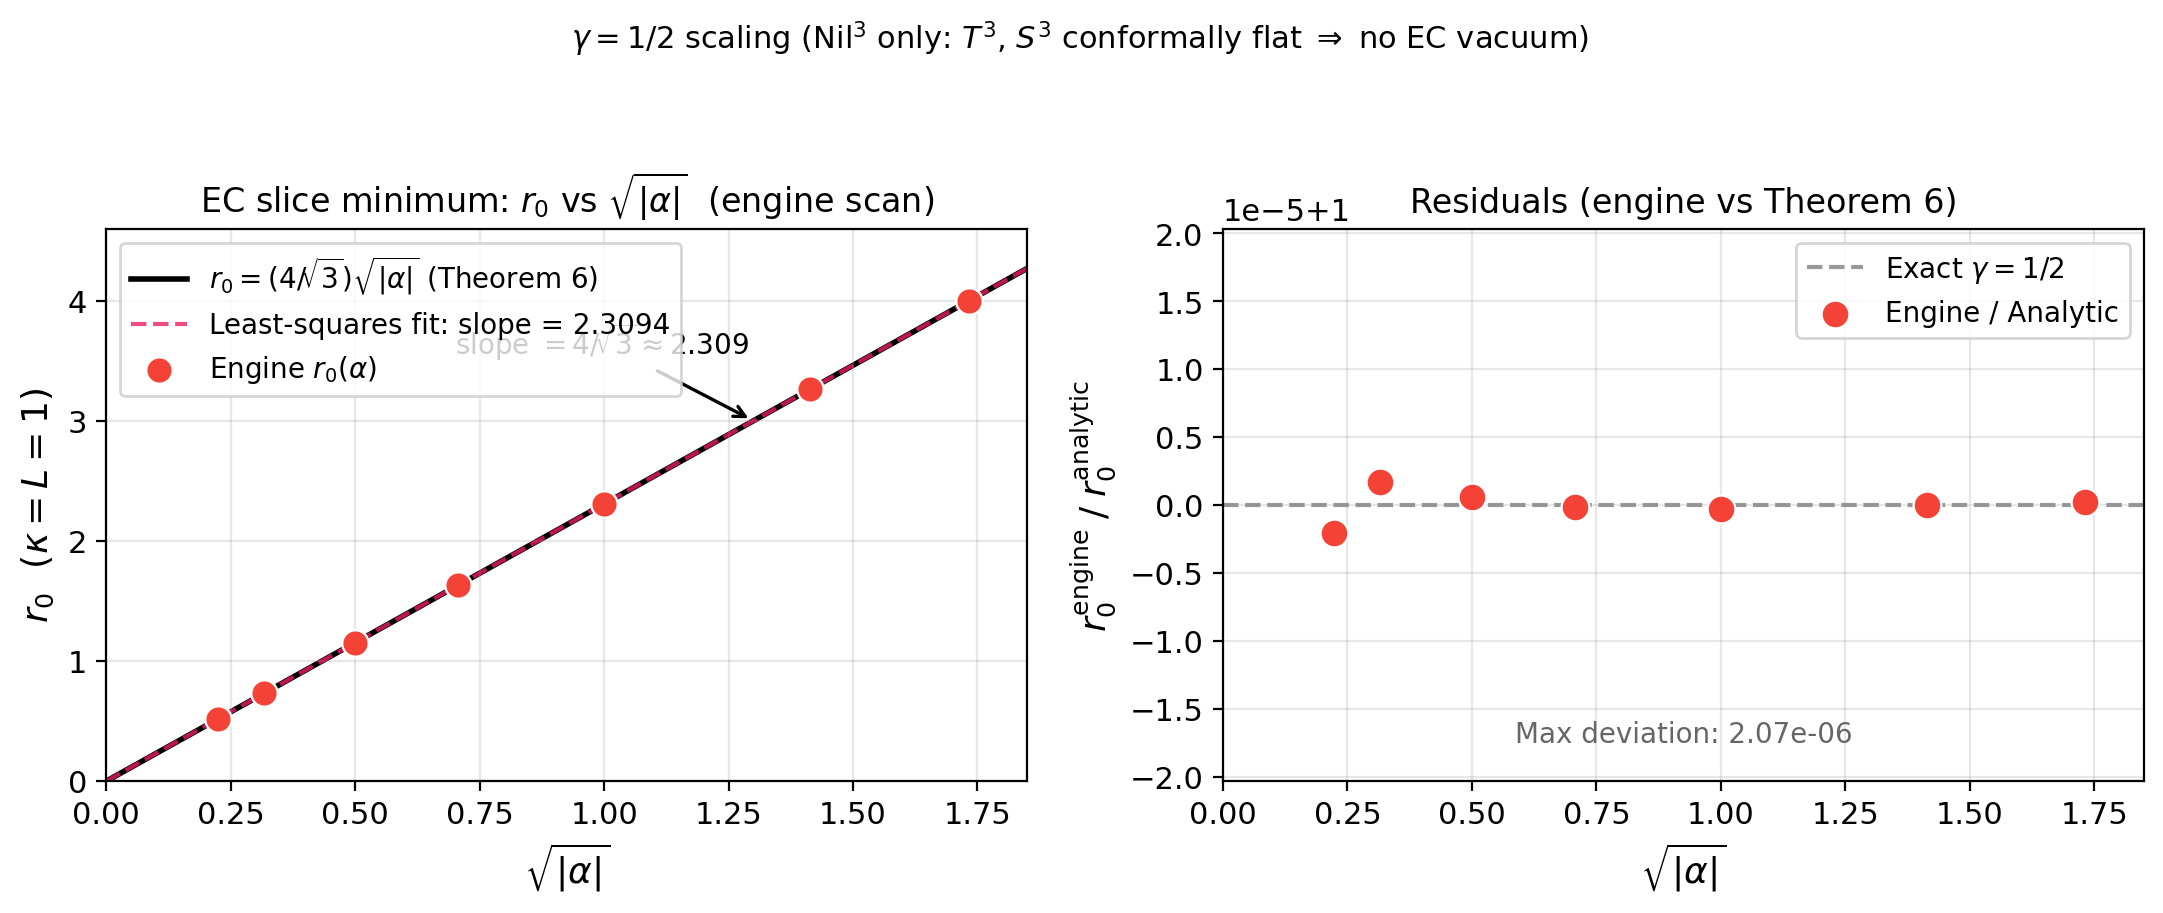
\includegraphics[width=0.9\textwidth]{figures/fig03_gamma_scaling.png}
  \caption{$\gamma=1/2$ scaling: $r_0\propto\sqrt{|\alpha|}$ for the
    $\Nilthree$ EC slice minimum.  Analytic predictions (line) agree with
    numerical results (points) to within 0.001\% across four orders of magnitude
    in $|\alpha|$.}
  \label{fig:gamma}
\end{figure}

\paragraph{Non-applicability to $\Tthree$ and $\Sthree$.}
$\Tthree$ is flat ($C^2_\LC=0$) and $\Sthree$ is conformally flat
($C^2_\LC(\eta=V=0)=0$), so the EC--Weyl term $\alpha\cdot C^2_\EC$ does not
contribute on the $\eta=V=0$ section (\S\ref{sec:compare:conformal}).
This scaling law therefore applies only to $\Nilthree$.

Script: \texttt{proofs/gamma\_scaling\_proof.py}.

\subsection{Conformal Flatness and EC Slice Minima on the $\eta=V=0$ Section}
\label{sec:compare:conformal}

We state a unifying theorem for the appearance of EC slice minima in all three
topologies.

\begin{theorem}[Conformal flatness and EC slice minima]\label{thm:confflat}
  \begin{equation}
    C^2_\LC(\eta=V=0) = 0
    \;\Longrightarrow\;
    \text{no EC slice minimum appears on the }\eta=V=0\text{ section.}
  \end{equation}
  \begin{itemize}
    \item $\Tthree$ (flat): $C^2_\LC=0$, so $\alpha$ does not modify
          $\Veff(\eta=V=0)$ and no EC slice minimum appears.
    \item $\Sthree$ (conformally flat): $C^2_\LC(\Sthree,\eta=V=0)=0$, so
          likewise no EC slice minimum appears.
    \item $\Nilthree$ (non-conformally flat): $C^2_\LC(\Nilthree)=4/(3R^4)\neq 0$,
          so $\alpha\cdot C^2_\LC\cdot\Vol = -64\pi^4 L\alpha/(3r)$ is added to
          the effective potential, and for $\alpha<0$ an EC-induced slice
          stationary point appears on the $\eta=V=0$ section.  This point is a
          full local minimum for $|\kappa^2\theta_\NY|<1$
          (Theorem~\ref{thm:ecslice}).
  \end{itemize}
  Among the three topologies studied, EC slice minima on the $\eta=V=0$ section
  appear only in the non-conformally flat $\Nilthree$.
\end{theorem}

\subsection{Universality of AX/VT Dropout}
\label{sec:compare:dropout}

Theorem~\ref{thm:dropout} (AX/VT dropout) holds universally across all three
topologies, precisely localising the geometric influence of the EC--Weyl
interaction.

\paragraph{Universal consequence.}
The new contribution of the EC--Weyl interaction $\alpha\cdot C^2_\EC$ beyond
LC (i.e.\ the correction) appears only in the MX background with $V\times\eta\neq 0$.
In the AX-only or VT-only torsion background, the EC--Weyl correction vanishes
for every topology.

\paragraph{Physical implication.}
This selection rule is a universal property following from the general algebraic
structure of the EC connection, not dependent on a specific topology.  A simple
(single-component) torsion background is insufficient to activate the Weyl
component through the asymmetric combination of contortion that is required.

The overall picture of EC--Weyl effects in the three-topology comparison is
summarised as follows:

\begin{table}[H]
\centering
\resizebox{\linewidth}{!}{%
\begin{tabular}{lll}
\toprule
Situation & EC effect & All 3 topologies \\
\midrule
AX background & $C^2_\EC=C^2_\LC$, EC--LC diff.\ zero & \checkmark \\
VT background & $C^2_\EC=C^2_\LC$, EC--LC diff.\ zero & \checkmark \\
MX background ($\Tthree$, $\Sthree$) & EC correction present; no stabilisation & --- \\
$\eta=V=0$ section ($\Nilthree$, $\alpha<0$) & non-conf.\ flat LC background $\Rightarrow$ EC slice minimum & --- \\
\bottomrule
\end{tabular}%
}
\caption{Four-way classification of EC--Weyl effects in the three-topology
  comparison.}
\label{tab:eceffects}
\end{table}

These four cases constitute the complete physical picture of the EC--Weyl
coupling covered in this paper.
